\documentclass[11pt]{article}

\usepackage[margin=1in]{geometry}
\usepackage{amsmath, amssymb, amsthm, bm}
\usepackage{booktabs}
\usepackage{graphicx}
\usepackage[numbers]{natbib}
\usepackage{hyperref}
\usepackage{microtype}

\newcommand{\NumPairs}{809}
\newcommand{\ImageSize}{120}
\newcommand{\BetaStart}{0.0005}
\newcommand{\BetaEnd}{0.1}
\newcommand{\NumSteps}{1000}
\newcommand{\FinalAlpha}{5.071e-12}
\newcommand{\FinalAlphaSq}{2.571e-23}
\newcommand{\EncodedSaturationPct}{65.7}
\newcommand{\EncodedRGBCorrelation}{-0.0006}
\newcommand{\RawAlphaMAE}{0.000000}
\newcommand{\ModelParamCount}{7,753,408}
\newcommand{\EncoderDatasetMAE}{0.00006691}
\newcommand{\DecoderDatasetMAE}{0.00395170}
\newcommand{\EncoderRGBMAE}{0.00008921}
\newcommand{\DecoderRGBMAE}{0.00526893}
\newcommand{\EncoderPSNR}{41.80}
\newcommand{\DecoderPSNR}{31.52}
\newcommand{\BaselineMAE}{0.25615245}
\newcommand{\BaselineRGBMAE}{0.34153659}
\newcommand{\BaselinePSNR}{5.75}
\newcommand{\EncoderExampleA}{bulbasaur}
\newcommand{\EncoderExampleB}{charizard}
\newcommand{\EncoderExampleC}{pikachu}
\newcommand{\EncoderExampleD}{mewtwo}

\graphicspath{{figures/}{../alshicrypt-multimodal.wiki/figures/}}

\newtheorem{proposition}{Proposition}

\title{\Large Learned Encrypter-Decrypter Models for Diffusion-Like Image Encryption:\\A Machine-Learning Approach Based on Stochastic Processes}
\author{Samuel Cavazos\\Alshival.AI}
\date{\today}

\begin{document}
\maketitle

\begin{abstract}
This paper documents a research prototype for learned image encryption based on a fixed stochastic forward process and paired neural endpoint maps. Starting from RGBA sprite images, we apply a diffusion-style corruption process to RGB channels while preserving alpha, then train one U-Net-like network to emulate the forward transform and a second network to learn its inverse. In this manuscript, the forward model is called the \emph{Encrypter} and the reverse model is called the \emph{Decrypter} to keep the transport framing explicit: the Encrypter is supposed to reproduce the distorted transit image, while the Decrypter is supposed to reconstruct the original image from that distorted input. The design was motivated by two practical observations: first, early experiments with deterministic non-linear tensor morphisms were difficult to generalize across images; second, stochastic corruption offers analytic control over signal attenuation, direct compatibility with one-step denoising ideas from consistency models, and a tunable bridge between structure preservation and information destruction.

The resulting system is successful as a research instrument: it trains stably, produces reproducible paired data, and learns low-error endpoint regressors on the current dataset. As a toy example, one can view the workflow as a machine-learning version of ``Who's That Pokemon?'': Mew is mapped to an obscured encrypted representation, transmitted in that form, and then reconstructed by a Decrypter at the receiving end, with the actual Decrypter output shown below rather than the original sprite reused as a placeholder. It is not yet a cryptosystem. For the default schedule used here, the pre-clipping signal coefficient after \NumSteps\ steps is only $\alpha_T=\FinalAlpha$, meaning that the RGB signal energy is effectively annihilated before clipping and quantization. Empirically, the final encrypted RGB values have correlation \EncodedRGBCorrelation\ with the source image and \EncodedSaturationPct\% of encrypted RGB channel values lie exactly at $0$ or $1$. The mathematical and empirical conclusion is that the current process is excellent for studying learned reconstruction under severe stochastic corruption, but exact reversibility and cryptographic security require stronger design constraints than those implemented in this prototype.

\begin{center}
    \setlength{\tabcolsep}{4pt}
    \begin{tabular}{ccccc}
        
\includegraphics[width=0.13\linewidth]{../pokemon/images/mew.png} &
        $\xrightarrow{\text{Encrypter}}$ &
        
\includegraphics[width=0.13\linewidth]{../pokemon_distorted/mew.png} &
        $\xrightarrow{\text{Decrypter}}$ &
        
\includegraphics[width=0.13\linewidth]{mew_decrypter_reconstruction.png} \\
        {\footnotesize Mew (Original)} && {\footnotesize Mew (Encrypted transit image)} && {\footnotesize Mew (Actual Decrypter reconstruction)}
    \end{tabular}
\end{center}

\begin{center}
    \textbf{Who's That Pokemon?}

    \vspace{4pt}
    \setlength{\tabcolsep}{8pt}
    \begin{tabular}{ccc}
        
\includegraphics[width=0.18\linewidth]{../pokemon_distorted/roselia.png} &
        
\includegraphics[width=0.18\linewidth]{../pokemon_distorted/vivillon.png} &
        
\includegraphics[width=0.18\linewidth]{../pokemon_distorted/claydol.png} \\
        {\footnotesize Mystery A} & {\footnotesize Mystery B} & {\footnotesize Mystery C}
    \end{tabular}

    \vspace{4pt}
    
    {\footnotesize Three distorted sprites from the dataset are shown above. Try to guess them before checking the answer key at the end of the paper.}
\end{center}
\end{abstract}

\section{Introduction}
This repository explores whether a machine-learning model pair can act like an Encrypter/Decrypter system for images after a deliberately destructive forward transform. The motivating application is not ordinary image compression; it is the stronger ambition of learning an \emph{encryption-like} transport mechanism in which a sender applies a difficult-to-interpret transformation and a receiver learns the inverse.

One long-term application class is privacy-sensitive image transport. In a future secure version of this framework, a sender-side model could encrypt a sensitive image, such as a radiology scan, pathology slide, or other healthcare image, into a transit representation that is difficult to interpret directly, send that representation over a network, and then use a receiver-side model to decrypt it after arrival. If that workflow were paired with keyed randomness and exact authorized recovery, it could complement conventional transport protections by reducing exposure of directly viewable patient content while images move between institutions or services. In that conceptual pipeline, ``encryption in transit'' refers to the middle stage, where only the encrypted representation is transmitted between endpoints. The original image remains at the sender, and the decrypted reconstruction appears only after the encrypted payload reaches the receiver. The current repository does not satisfy the security, reversibility, or regulatory requirements for protected health information; here the healthcare example is a motivating application target, not a claim of deployment readiness.

Our early internal experiments focused on deterministic non-linear tensor morphisms: handcrafted non-linear spatial and channel transforms designed to scramble image tensors without explicit randomness. In practice, these morphisms were difficult to generalize. They often behaved like brittle texture-specific warps: they could fit seen patterns, but they did not produce a clean family of transformations with obvious scaling laws or analytically controlled information loss. That experience motivated a shift toward a stochastic process.

The stochastic choice was informed by diffusion and consistency-model literature. Diffusion models are attractive because the forward corruption process is mathematically tractable, the signal-to-noise tradeoff is tunable through a schedule, and a learned network can target endpoint recovery instead of inverting an arbitrary handcrafted morphism \citep{ho2020ddpm, song2021sde, song2023consistency}. Our prototype adopts that philosophy in a simplified supervised form: generate paired samples with a fixed stochastic process, then learn direct maps for the forward and reverse endpoints.

\paragraph{Contributions.}
This paper makes four concrete contributions:
\begin{enumerate}
    \item It formalizes the current stochastic forward transform and derives its closed-form endpoint distribution before clipping.
    \item It explains why a stochastic path was chosen over deterministic non-linear tensor morphisms for this line of work.
    \item It reports the empirical behavior of the current repository implementation, including quantitative distortion statistics, endpoint training curves, and qualitative reconstructions.
    \item It identifies the precise gap between the current prototype and a true cryptographic system.
\end{enumerate}

\section{Background and Motivation}
\subsection{Images as functions and the endomorphism viewpoint}
We can formalize the data domain at the pixel level. Let
\begin{equation}
A = [0,1]^4
\end{equation}
denote the normalized RGBA attribute space of a single pixel. Let $\Omega$ denote a finite coordinate grid. An image can then be viewed as a function
\begin{equation}
i : \Omega \to A,
\end{equation}
which assigns an RGBA value to each coordinate.

This perspective suggests an algebraic design target for learned transport. Rather than beginning with a full image-to-image black box, we can seek an endomorphism
\begin{equation}
F : A \to A
\end{equation}
that distorts pixel values while remaining invertible by construction, and then induce an image-level operator coordinatewise:
\begin{equation}
(\mathcal{F}i)(u) = F(i(u)), \qquad u \in \Omega.
\end{equation}
In the idealized setting, the sender applies $\mathcal{F}$ and the receiver applies $\mathcal{F}^{-1}$, while machine-learning models are trained to approximate $F$ and $F^{-1}$ from data.

The same viewpoint is not limited to images. Once a medium is represented as a function from an index set into a local attribute space, the same endomorphism idea extends naturally to other modalities. For example, audio can be modeled as a function from time indices to amplitude values or short local feature vectors, and an invertible endomorphism on that value space would induce an analogous encrypt/decrypt operator for sound.

This paper studies one stochastic route toward that broader objective. In the current public prototype, all tensors are normalized to $[0,1]$ during processing and learning. The implemented endpoint map is diffusion-like and analytically tractable before clipping and quantization, but the stored PNG pipeline is not exactly invertible. The endomorphism framing is therefore best understood here as the conceptual target for the research program, rather than as a property already achieved by the released implementation.

\subsection{Tensor algebra as the broader category-theoretic framing}
The image-as-function viewpoint is useful because it exposes the image case cleanly, but the broader research program is better expressed one level up in tensor algebra. In that broader view, image and audio examples are best understood as concrete cases that help us study and understand the framework, not as the boundary of the framework itself. Instead of privileging coordinates first, we can regard a modality sample as a tensor
\begin{equation}
x \in V,
\end{equation}
where $V$ is a modality-specific tensor space. For the current repository, $V$ is the space of normalized RGBA image tensors; in future instances, $V$ could instead be an audio waveform space, a spectrogram space, a token-embedding tensor space for text, or another tensorized data domain. The point of the formulation is to generalize across modalities, with image and audio serving as especially intuitive cases for building understanding.

In that formulation, the encryption algorithm is modeled as a tensor morphism
\begin{equation}
T : V \to V.
\end{equation}
The learned forward and reverse networks are then interpreted as learned tensor maps
\begin{equation}
E : V \to V,
\qquad
D : V \to V,
\end{equation}
with the intended relationships
\begin{equation}
E(x) \approx T(x),
\qquad
D(E(x)) \approx x.
\end{equation}
This is the category-theoretic version of the endomorphism viewpoint for the encryption algorithm: the same abstract pattern can be instantiated across multiple modalities as long as the data admit a tensor representation.

\begin{figure}[t]
    \centering
    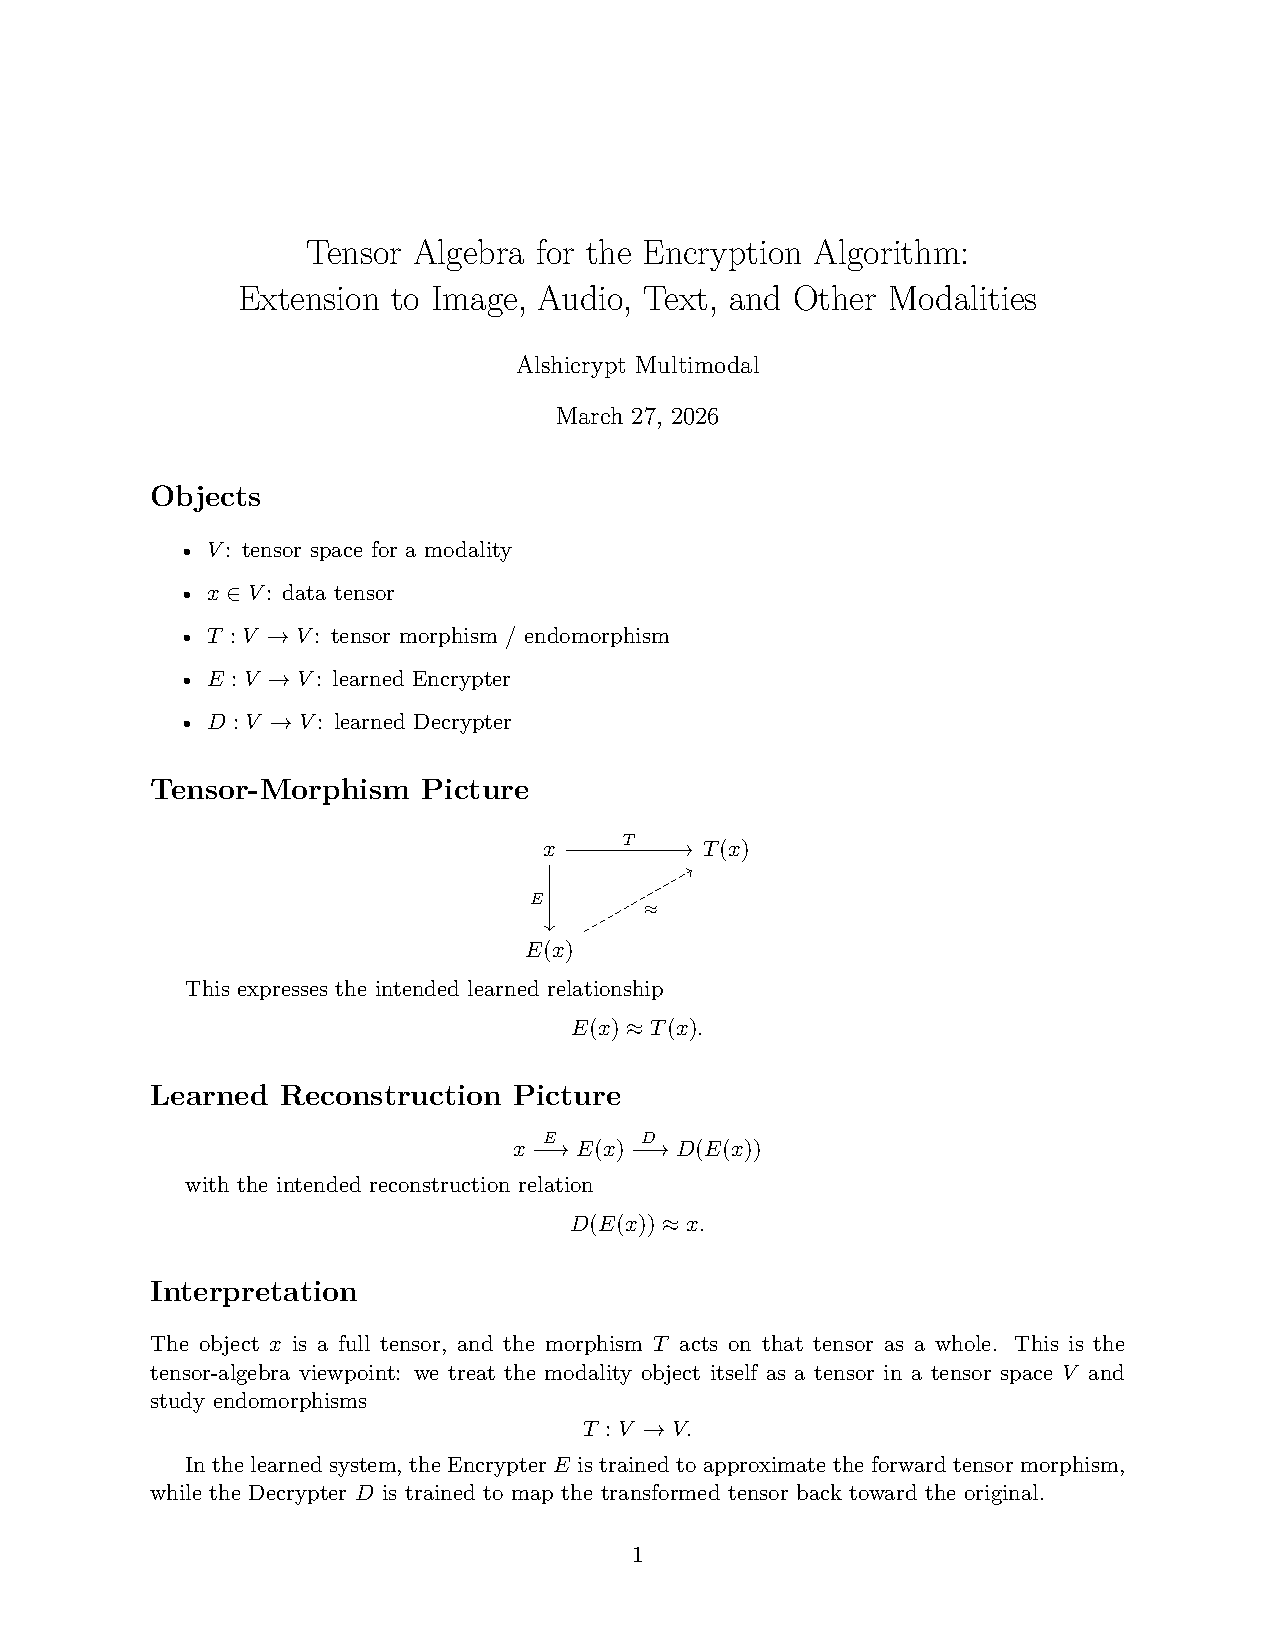
\includegraphics[width=0.82\linewidth]{../category_theory.pdf}
    \caption{Tensor-algebra view of the encryption algorithm. A modality sample is treated as a tensor $x \in V$, the intended encryption transform is a tensor morphism $T : V \to V$, and the learned Encrypter $E$ and Decrypter $D$ are trained to approximate the forward and reverse tensor maps. The current repository instantiates this picture for image tensors; image and audio cases are especially useful for intuition, but the abstraction is meant to generalize to text and other tensor-representable modalities as well.}
    \label{fig:tensor-algebra-view}
\end{figure}

This tensor-space abstraction clarifies why the current image results matter beyond images themselves. The immediate contribution of the repository is an image-tensor instantiation, but the larger idea is a modality-agnostic encryption/decryption program built from endomorphisms on tensor spaces. In that sense, image and audio should be read as understanding-generating examples of the formalism, whereas the research target is a transferable framework that can be adapted to many kinds of modality.

\subsection{Why stochastic corruption is attractive}
Let $x_0 \in [0,1]^{H \times W \times 4}$ denote a normalized RGBA image. A deterministic tensor morphism seeks a map
\begin{equation}
z = g(x_0),
\end{equation}
where $g$ is intentionally hard to interpret yet still invertible or approximately invertible. The problem is that once $g$ becomes sufficiently non-linear to hide semantics, it typically becomes difficult to characterize globally. Local Jacobians can vary sharply across the image manifold, and small changes in spatial structure may produce qualitatively different outputs. In our exploratory work this made generalization brittle.

By contrast, a stochastic process defines a family of transforms indexed by noise variables:
\begin{equation}
z = T_{\omega}(x_0),
\end{equation}
where $\omega$ denotes a random seed or noise path. This has three advantages.

First, the endpoint distribution can often be analyzed exactly or approximately. Second, the process difficulty can be tuned continuously by a schedule rather than redesigned from scratch. Third, the same corrupted endpoint can be paired with direct learned maps, echoing the endpoint-consistency view that motivates one-step generation and denoising in consistency models \citep{song2023consistency}.

\subsection{Relation to consistency models}
Consistency models learn functions that map points on a noise path toward a shared consistent output, allowing high-quality generation in very few steps \citep{song2023consistency}. Our method is not a consistency model in the strict sense: we do not train across multiple times with a consistency objective, nor do we solve the probability-flow ODE used in that work. The connection is conceptual rather than identical. The consistency-model literature encouraged us to prefer a stochastic path with analyzable marginals and to investigate whether direct endpoint maps can work without iterative reverse sampling.

\section{Method}
\subsection{Data domain}
The current repository uses \NumPairs\ Pokemon sprite pairs as a controlled RGBA image dataset. Let
\begin{equation}
x_0 = (r_0, g_0, b_0, a_0) \in [0,1]^{H \times W \times 4}.
\end{equation}
Here all channels are normalized to $[0,1]$ tensors before processing. The RGB channels are treated as the signal to corrupt; the alpha channel is preserved exactly in the current implementation.

\subsection{Forward process}
Define $y_t \in \mathbb{R}^{H \times W \times 3}$ as the RGB state at step $t$, with $y_0 = (r_0,g_0,b_0)$. Let $\varepsilon_t$ denote independent standard Gaussian noise over the flattened RGB coordinates, so $\operatorname{vec}(\varepsilon_t) \sim \mathcal{N}(0, I_{3HW})$. The forward process implemented in the repository is
\begin{equation}
y_t = \sqrt{1-\beta_t}\, y_{t-1} + \sqrt{\beta_t}\, \varepsilon_t,
\label{eq:forward}
\end{equation}
for $t=1,\dots,T$, where $T=\NumSteps$ and the schedule is linearly interpolated from $\beta_1=\BetaStart$ to $\beta_T=\BetaEnd$.

The stored encoded image is then
\begin{equation}
z = \bigl(Q(\operatorname{clip}(y_T, 0, 1)), a_0\bigr),
\label{eq:stored}
\end{equation}
where $\operatorname{clip}$ clamps each RGB value to $[0,1]$ and $Q$ denotes 8-bit PNG quantization.

\paragraph{Implementation note.}
For reproducible paired supervision, the current public prototype uses a fixed pseudorandom realization during dataset generation. In other words, the \emph{family} is stochastic, but the released dataset corresponds to one realized corruption path. This is useful for supervised learning and reproducibility, but it is weaker than a deployment setting with keyed per-message randomness.

\subsection{Learned endpoint maps}
Two separate neural networks are trained:
\begin{align}
f_{\theta_e} &: x_0 \mapsto z, \\
f_{\theta_d} &: z \mapsto x_0.
\end{align}
In repository code and CLI flags these stages are still named `encoder' and `decoder' for backward compatibility, but in the paper we refer to $f_{\theta_e}$ as the \emph{Encrypter} and $f_{\theta_d}$ as the \emph{Decrypter}. Both are instantiated as the same compact U-Net-like CNN with \ModelParamCount\ trainable parameters, built from three downsampling blocks, a bottleneck, and three decoder blocks with skip connections following the U-Net design pattern \citep{ronneberger2015unet}.

Training uses an $L_1$ objective:
\begin{align}
\mathcal{L}_{\text{enc}}(\theta_e) &= \frac{1}{N}\sum_{i=1}^{N} \left\lVert f_{\theta_e}(x_0^{(i)}) - z^{(i)} \right\rVert_1, \\
\mathcal{L}_{\text{dec}}(\theta_d) &= \frac{1}{N}\sum_{i=1}^{N} \left\lVert f_{\theta_d}(z^{(i)}) - x_0^{(i)} \right\rVert_1.
\end{align}
The repository reports dataset mean absolute error (MAE), which is the elementwise absolute error averaged over every pixel and channel.

\section{Mathematical Analysis}
\subsection{Closed-form endpoint distribution}
Equation~\eqref{eq:forward} is a discrete-time linear Gaussian process on RGB pixels. Define
\begin{equation}
\alpha_t = \prod_{s=1}^{t} \sqrt{1-\beta_s}.
\end{equation}

\begin{proposition}
Conditioned on $y_0$, the pre-clipping endpoint distribution is
\begin{equation}
\operatorname{vec}(y_t) \mid y_0 \sim \mathcal{N}\!\left(\alpha_t \operatorname{vec}(y_0),\; (1-\alpha_t^2)I_{3HW}\right).
\end{equation}
\end{proposition}

\begin{proof}
Unrolling Equation~\eqref{eq:forward} yields
\begin{equation}
y_t = \alpha_t y_0 + \sum_{k=1}^{t} \left( \sqrt{\beta_k} \prod_{s=k+1}^{t} \sqrt{1-\beta_s} \right)\varepsilon_k.
\end{equation}
The mean conditioned on $y_0$ is therefore $\alpha_t y_0$. Since the $\varepsilon_k$ are independent standard Gaussians over the flattened RGB coordinates, the covariance is the sum of the squared coefficients:
\begin{equation}
\sum_{k=1}^{t} \beta_k \prod_{s=k+1}^{t} (1-\beta_s)
 = 1 - \prod_{s=1}^{t} (1-\beta_s)
 = 1 - \alpha_t^2.
\end{equation}
Thus $\operatorname{vec}(y_t) \mid y_0$ is Gaussian with the claimed mean and covariance.
\end{proof}

\subsection{Why the chosen schedule is so destructive}
For the default schedule, the final attenuation coefficient is
\begin{equation}
\alpha_T = \FinalAlpha,
\qquad
\alpha_T^2 = \FinalAlphaSq.
\end{equation}
This means the linear signal energy surviving in RGB at step $T$ is effectively zero before clipping. The forward process therefore behaves almost like pure Gaussian noise at the endpoint, after which clipping and 8-bit quantization collapse many distinct continuous states into the same stored PNG values.

Figure~\ref{fig:forward-process} makes this explicit. The linear schedule increases noise steadily, while the surviving signal coefficient decays superlinearly in log scale.

\begin{figure}[t]
    \centering
    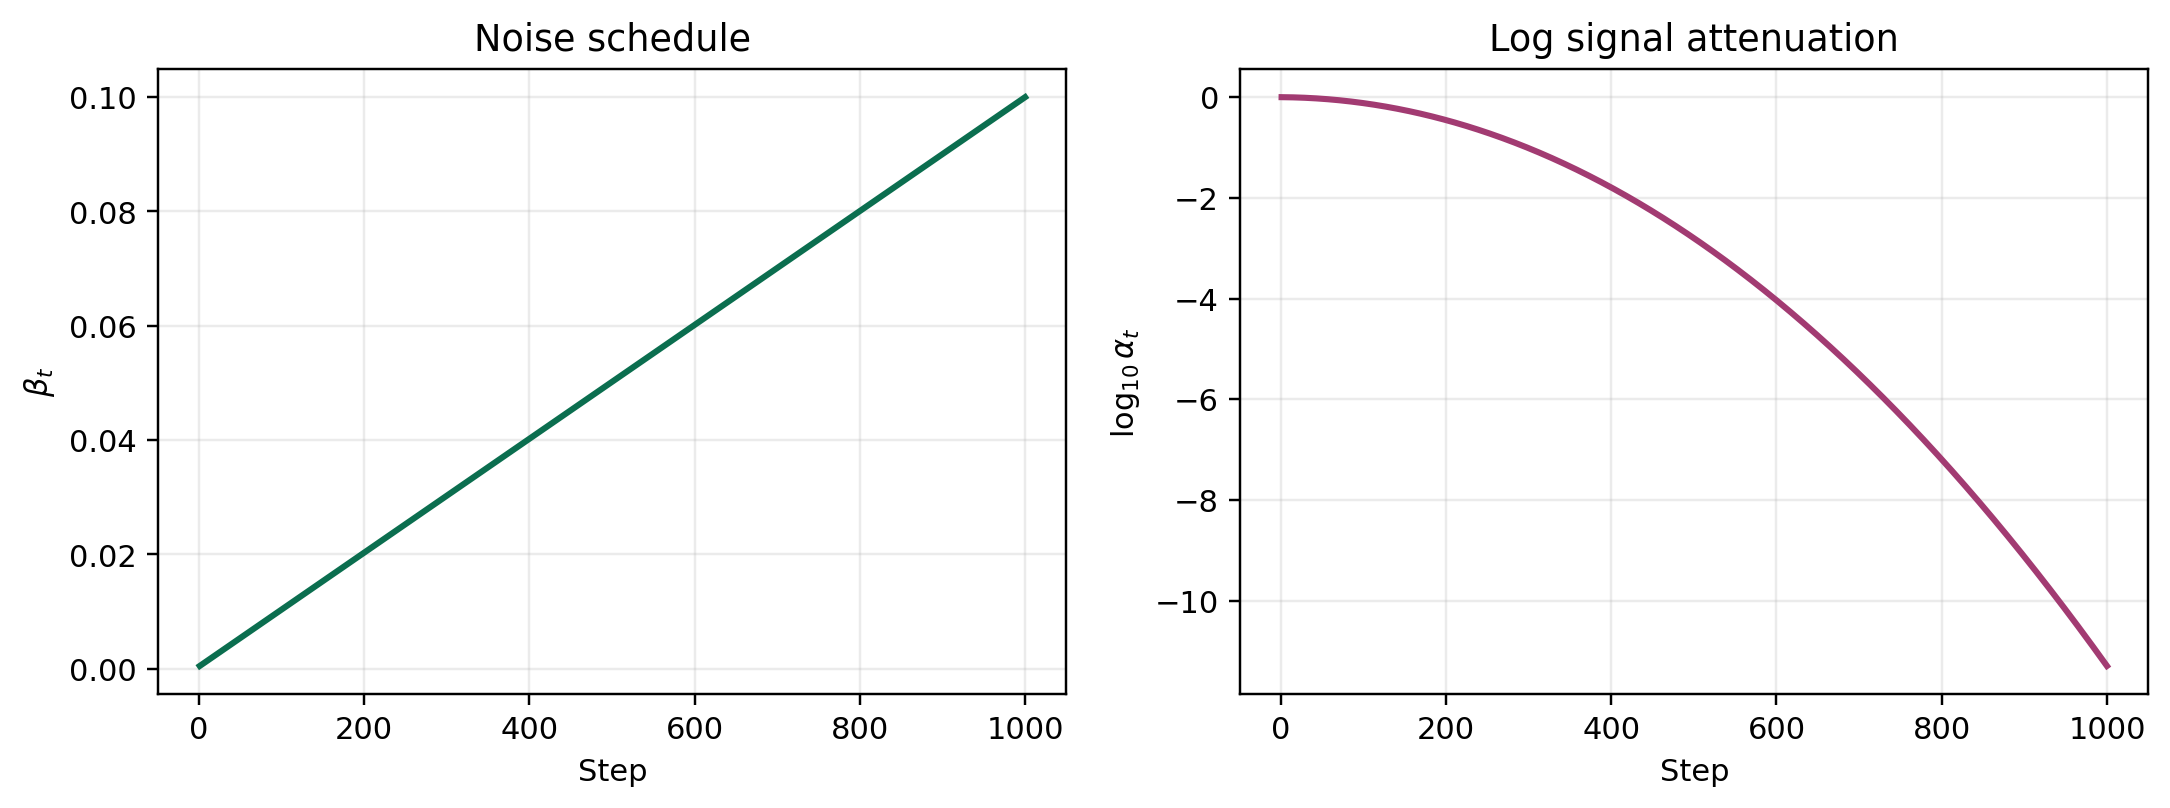
\includegraphics[width=\linewidth]{forward_process.png}
    \caption{The default corruption schedule used in the repository. Left: the linear $\beta_t$ schedule. Right: the log attenuation coefficient $\log_{10}\alpha_t$. By the final step, the RGB signal contribution is effectively annihilated.}
    \label{fig:forward-process}
\end{figure}

\subsection{Implications for invertibility}
The current forward operator is not injective once clipping and quantization are applied. Even if two distinct source images $x_0 \neq x_0'$ induce different continuous distributions before quantization, the map in Equation~\eqref{eq:stored} collapses broad regions of RGB space to the same 8-bit values. Exact inversion is therefore impossible in general.

This is the central mathematical distinction between our prototype and a cryptosystem. A cryptosystem can be computationally hard to invert without a key while still being exactly invertible with the key. The present process is instead \emph{information-destroying}. Recovery must therefore come from learned image priors and dataset regularity, not from formal reversibility.

\subsection{Role of alpha preservation}
The alpha channel is preserved exactly in the dataset generator, so the raw alpha-channel MAE between original and encoded images is \RawAlphaMAE. This matters for interpretation. A zero-error alpha channel lowers aggregate MAE while leaving RGB corruption unchanged. Consequently, RGB-only MAE is the more informative statistic when discussing semantic recovery.

\section{Experimental Setup}
The public experiment uses the repository's current configuration:
\begin{itemize}
    \item Dataset size: \NumPairs\ paired images.
    \item Image resolution during training: $\ImageSize \times \ImageSize$ RGBA.
    \item Forward schedule: $\NumSteps$ steps, linear $\beta_t$ from \BetaStart\ to \BetaEnd.
    \item Architecture: U-Net-like CNN with \ModelParamCount\ trainable parameters.
    \item Objective: elementwise $L_1$ loss.
    \item Training logs used here: 100-epoch Encrypter and Decrypter runs from the repository's `models/paper\_eval` directory.
\end{itemize}

These are training-set results, not holdout results. They are useful for understanding whether the endpoint maps can fit the current paired transformation, but they should not be interpreted as evidence of security or strong out-of-distribution generalization.

\section{Results}
\subsection{Forward-process statistics}
The encoded RGB endpoint is heavily saturated and nearly decorrelated from the source RGB. Across the current dataset:
\begin{itemize}
    \item \EncodedSaturationPct\% of encoded RGB values are exactly 0 or 1 after clipping and quantization.
    \item The flattened RGB correlation between source and encoded images is \EncodedRGBCorrelation.
    \item The alpha channel is unchanged.
\end{itemize}

This validates the intended behavior of the stochastic transform: the visible endpoint is hard to interpret directly. It also explains why exact inversion is mathematically impossible in the current design.

\subsection{Training behavior}
Both endpoint networks train smoothly over the first 20 epochs, with monotone decreases in train $L_1$ and dataset MAE. Figure~\ref{fig:training-curves} shows that the Decrypter converges slightly better than the Encrypter on this dataset.

\begin{figure}[t]
    \centering
    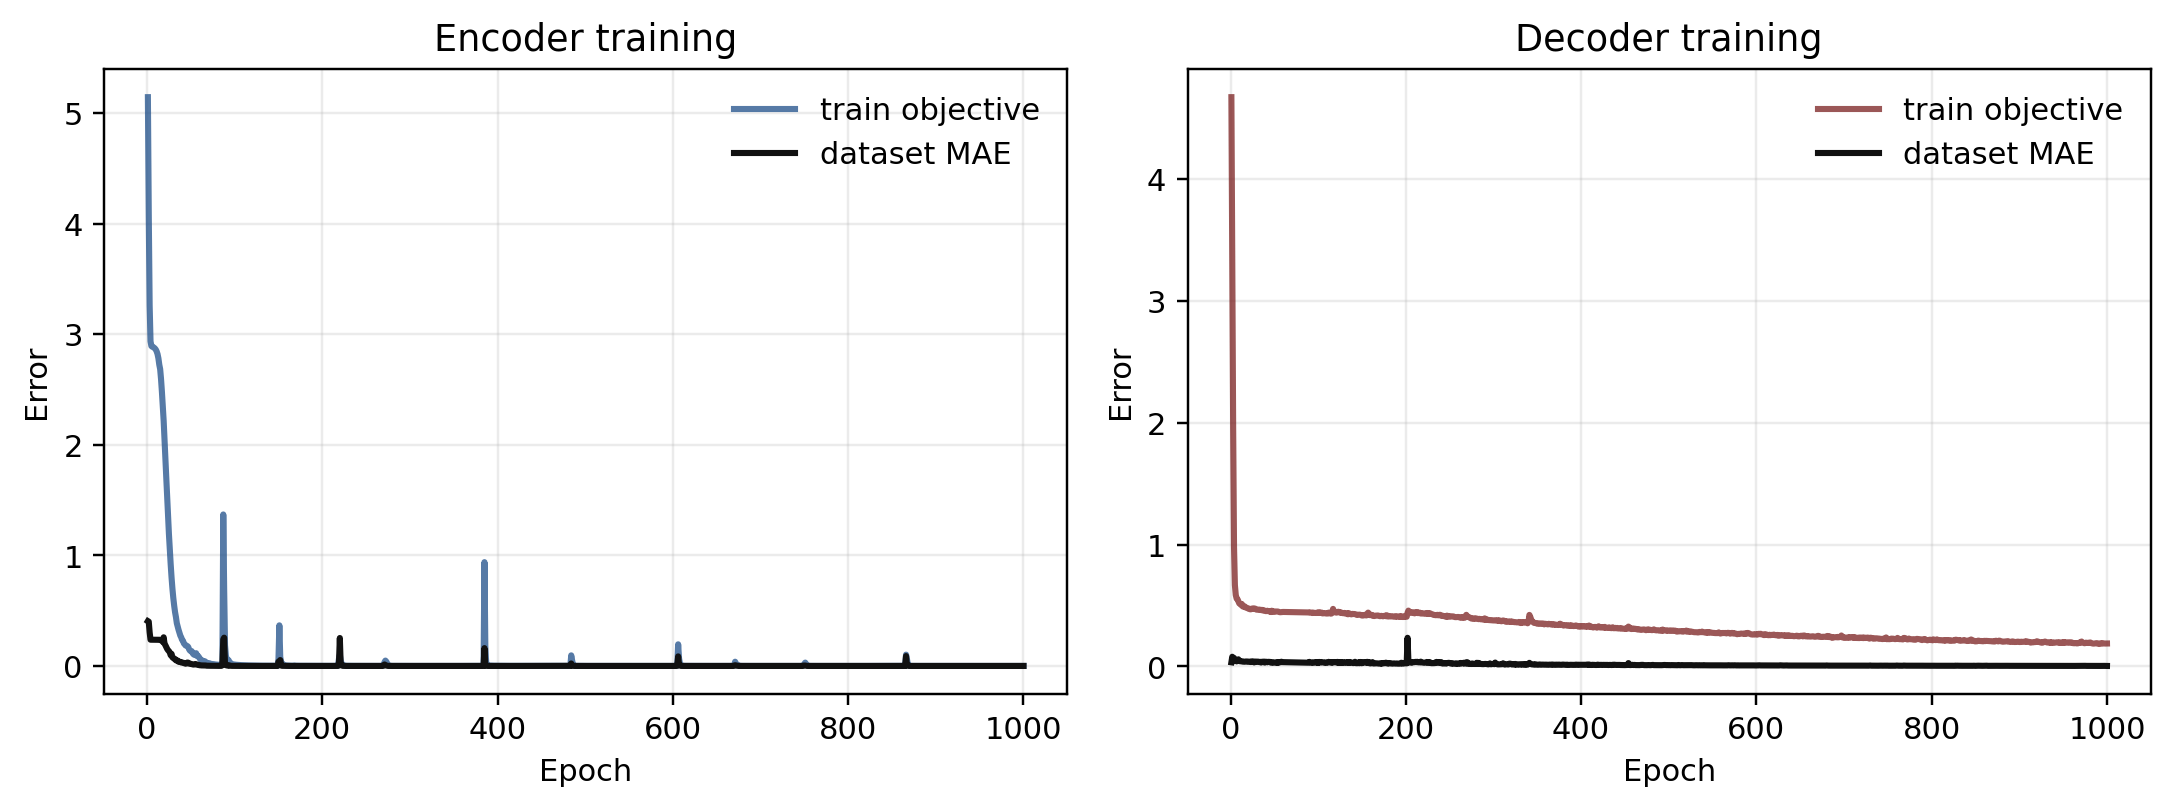
\includegraphics[width=\linewidth]{training_curves.png}
    \caption{Training dynamics for the Encrypter and Decrypter endpoint networks. Both optimize stably, supporting the claim that the stochastic pairing setup is learnable even with a relatively small convolutional model.}
    \label{fig:training-curves}
\end{figure}

\subsection{Quantitative endpoint accuracy}
Table~\ref{tab:main-results} summarizes the main quantitative results. The direct baseline compares the original image to the encoded image without a learned model. Both learned models improve substantially over that baseline.

\begin{table}[t]
    \centering
    \begin{tabular}{lccc}
        \toprule
        Metric & Direct baseline & Encrypter & Decrypter \\
        \midrule
        All-channel MAE & \BaselineMAE & \EncoderDatasetMAE & \DecoderDatasetMAE \\
        RGB-only MAE & \BaselineRGBMAE & \EncoderRGBMAE & \DecoderRGBMAE \\
        RGB PSNR (dB) & \BaselinePSNR & \EncoderPSNR & \DecoderPSNR \\
        \bottomrule
    \end{tabular}
    \caption{Dataset-level endpoint metrics on the current paired dataset. All-channel MAE is lower than RGB-only MAE because alpha is preserved exactly by the forward generator.}
    \label{tab:main-results}
\end{table}

\subsection{Qualitative behavior}
Figure~\ref{fig:reconstruction-grid} illustrates the current visual behavior. The encrypted targets are visually noisy and semantically obscured. The Encrypter should therefore be judged by how closely it matches that distorted transit target, not by similarity to the original image. The learned Encrypter now tracks the distorted target closely, including much of its clipped color distribution. The Decrypter recovers recognizable geometry and smooth tonal structure, but color fidelity remains limited and the outputs are still visibly softer than the originals.

\begin{figure}[t]
    \centering
    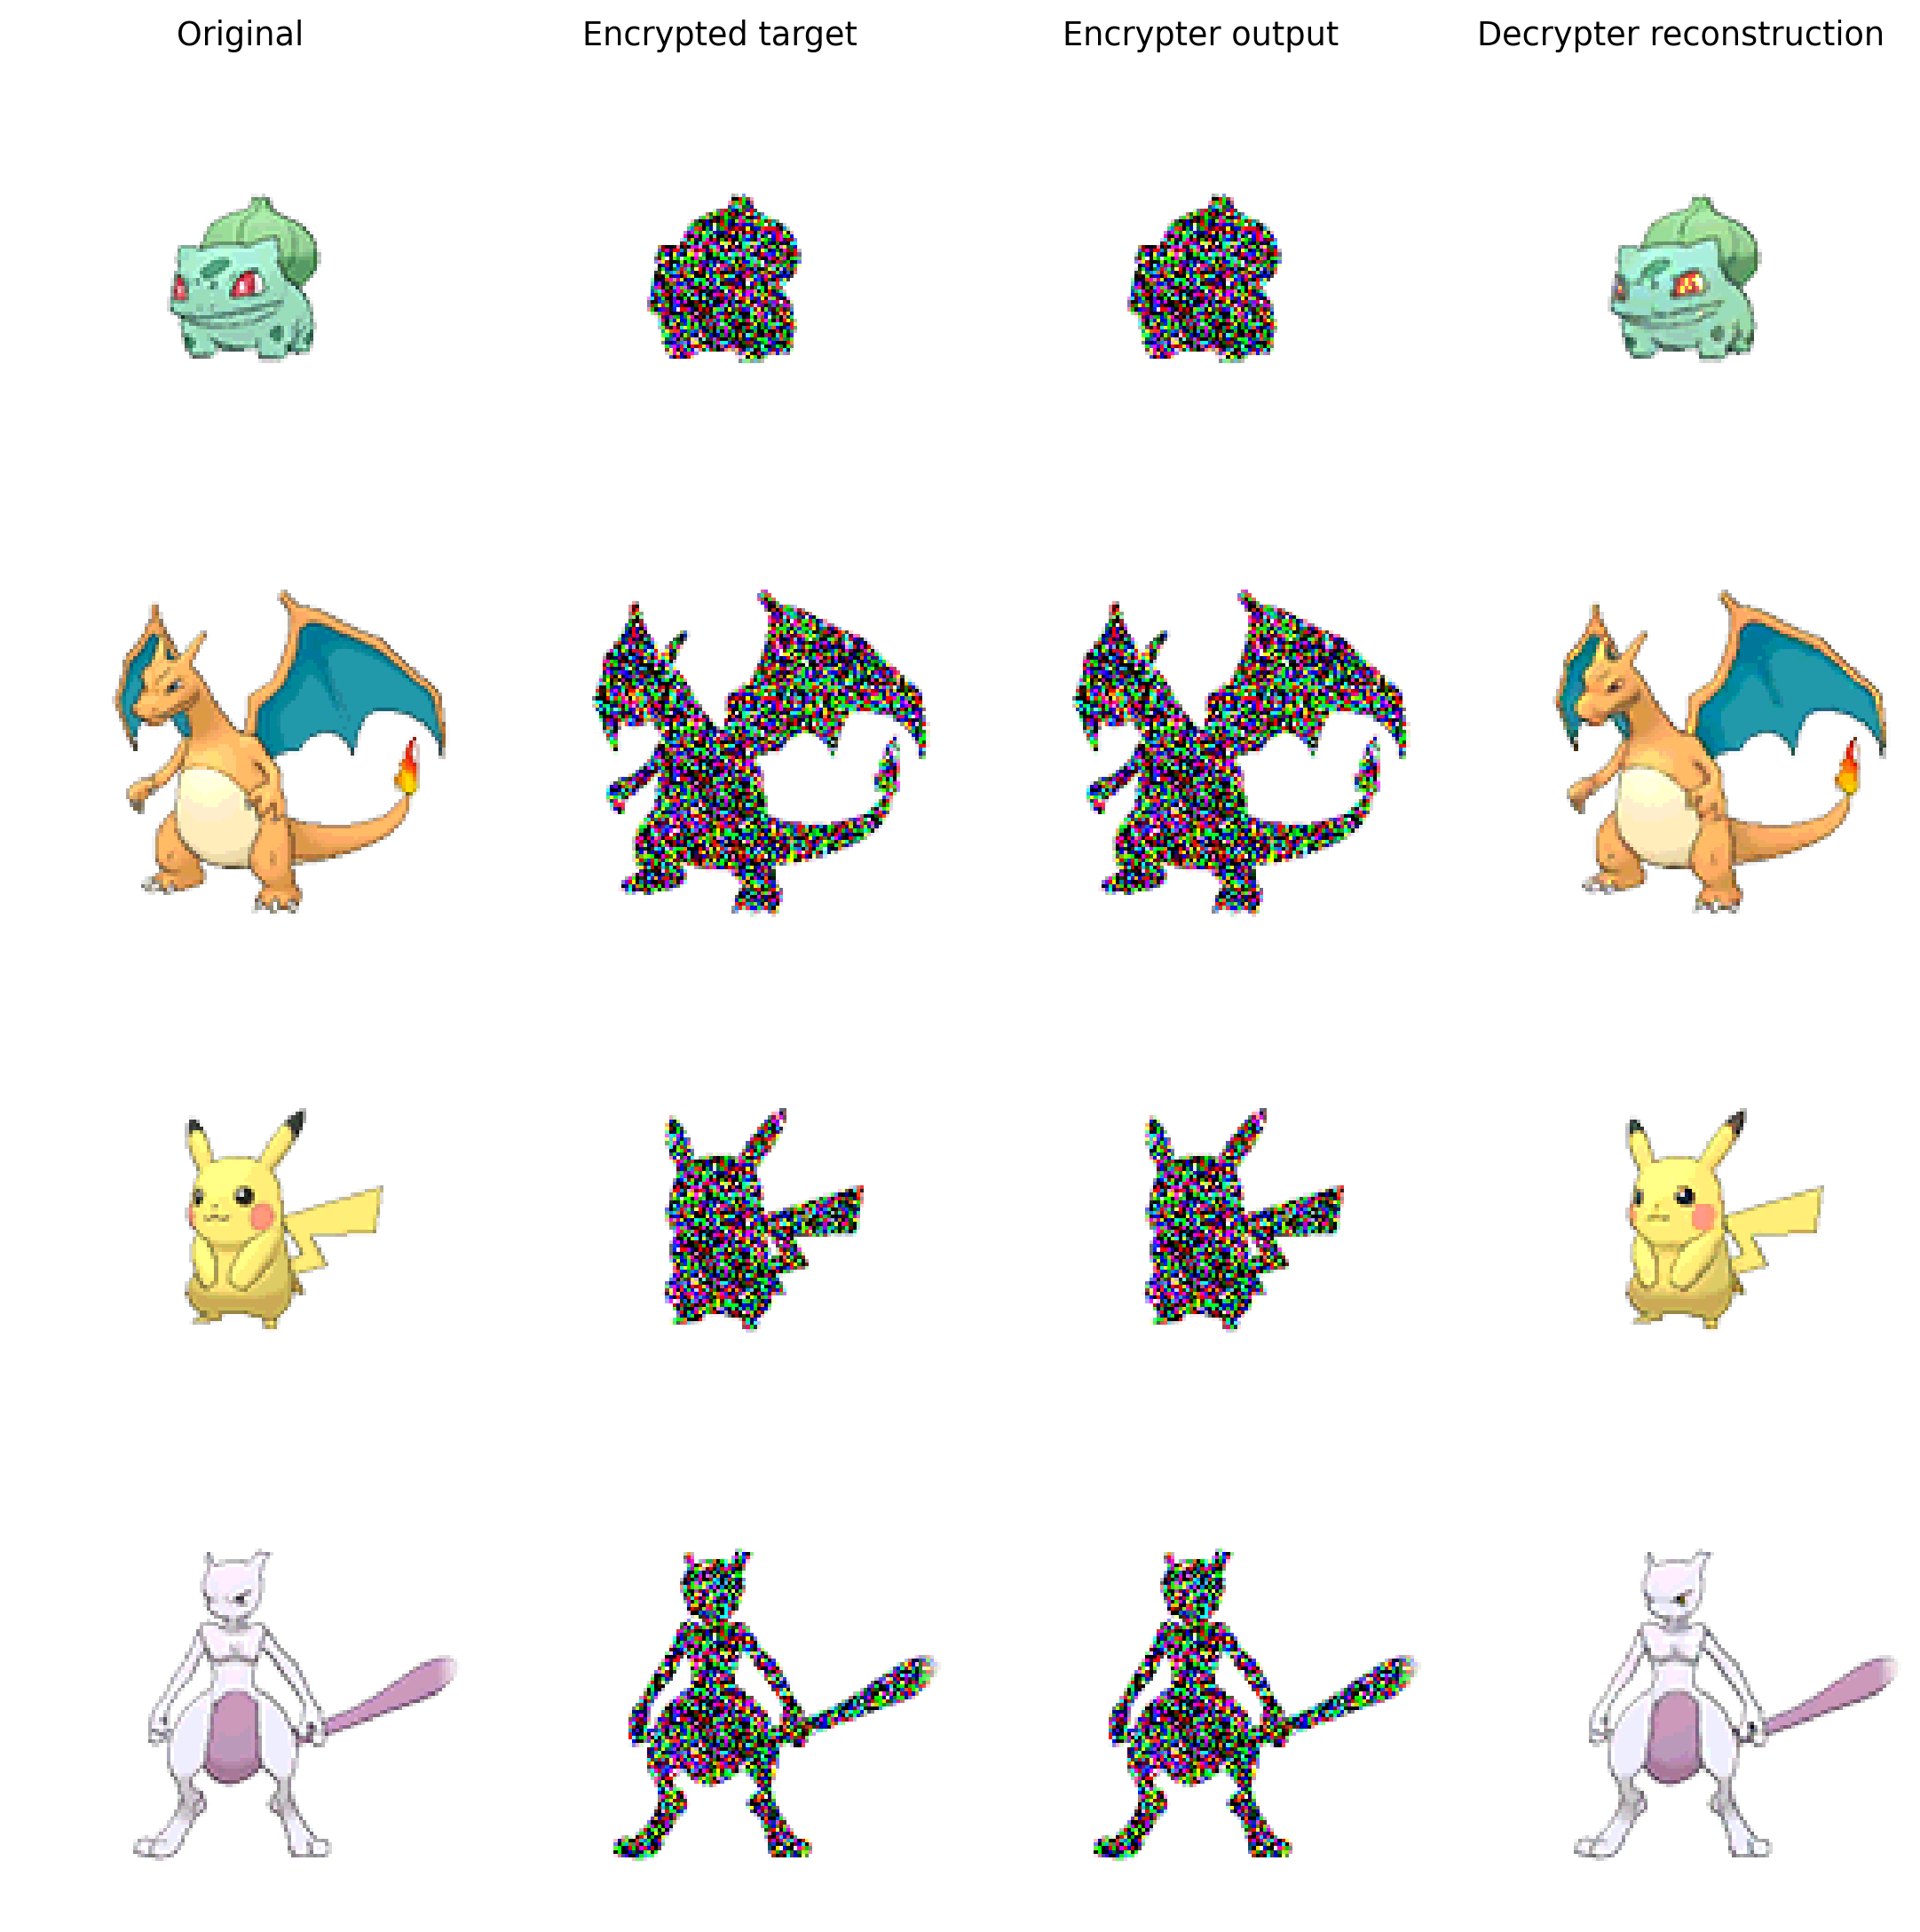
\includegraphics[width=\linewidth]{reconstruction_grid.png}
    \caption{Qualitative examples from the current repository checkpoints: \EncoderExampleA, \EncoderExampleB, \EncoderExampleC, and \EncoderExampleD. Left-to-right within each example, the Encrypter output is supposed to resemble the distorted encrypted target rather than the original image. The final column is the Decrypter reconstruction from that encrypted input. The new paper checkpoints recover geometry and some smooth shading reliably, although the reconstructions remain softer and less colorful than the originals.}
    \label{fig:reconstruction-grid}
\end{figure}

Figure~\ref{fig:pixel-statistics} reinforces the same conclusion. The encoded RGB distribution is sharply concentrated at clipped values, and the learned models reduce error against the direct baseline but do not recover a truly invertible channel.

\begin{figure}[t]
    \centering
    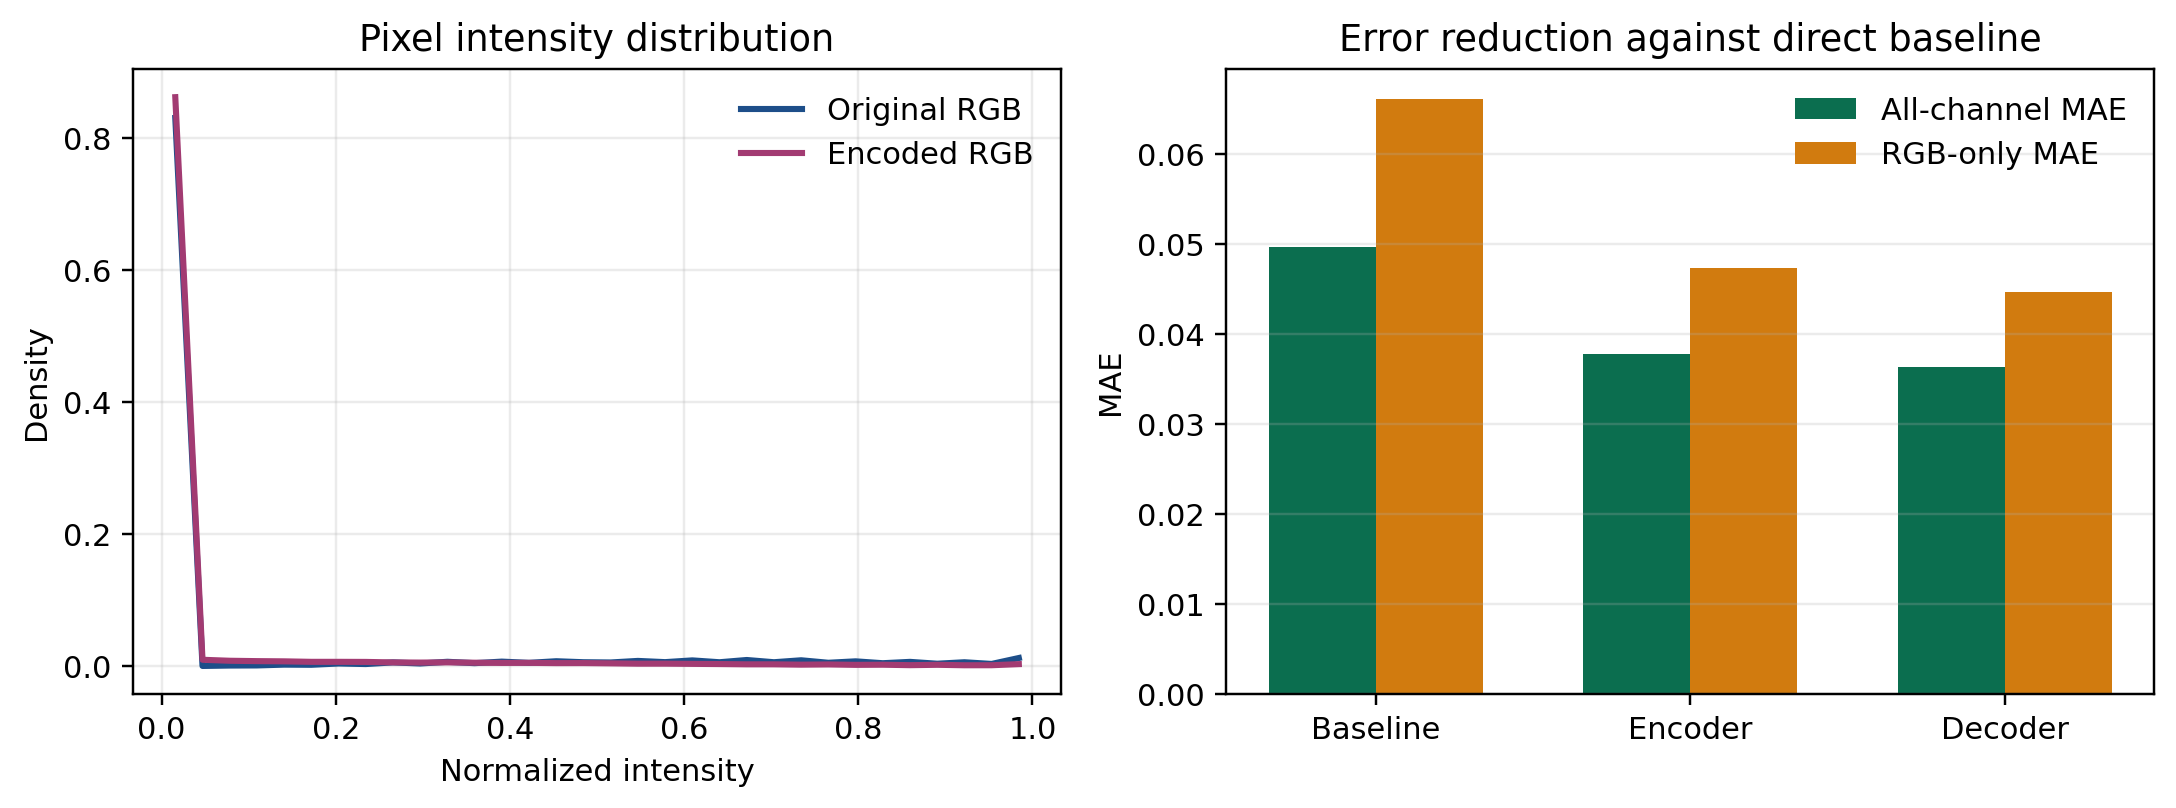
\includegraphics[width=\linewidth]{pixel_statistics.png}
    \caption{Left: original and encrypted RGB intensity distributions. Right: error reduction relative to the direct baseline. The current Decrypter improves over the baseline, but the improvement is incremental rather than evidence of full reversibility.}
    \label{fig:pixel-statistics}
\end{figure}

\section{Discussion}
\subsection{What succeeded}
The stochastic reformulation solved several problems that appeared in the earlier deterministic-morphism stage of this project.

First, it gave the experiment a mathematically transparent forward path. Second, it produced a stable supervised learning problem with direct paired targets. Third, it enabled one-step learned endpoint maps that train cleanly with a simple convolutional architecture. These are meaningful successes for a research prototype.

\subsection{What failed, or remains unresolved}
Three limitations are structural rather than incidental.

\paragraph{The process is not reversible.}
Because clipping and quantization destroy information, the Decrypter is solving an image-reconstruction problem under a strong prior, not decrypting a formally invertible ciphertext.

\paragraph{The current implementation leaks alpha.}
Preserving alpha means one quarter of the channels are already solved. This lowers aggregate error and exposes silhouette information directly.

\paragraph{The public prototype fixes a single realized corruption path.}
That choice is appropriate for reproducible training pairs, but it is not a secure keyed scheme. A production-grade system would need secret per-message randomness or a keyed pseudorandom generator driving the corruption schedule.

\subsection{Why the stochastic choice was still the right research move}
Despite those limitations, the stochastic choice was justified. It gave us an analyzable corruption operator, a well-conditioned training target, and a direct way to study the gap between \emph{learned reconstruction under noise} and \emph{cryptographic reversibility}. Deterministic non-linear tensor morphisms did not provide that level of control or transparency in our exploratory work.

The tensor-algebra framing in Figure~\ref{fig:tensor-algebra-view} also helps explain why this remains a useful research direction despite the present limitations. Even though the current public implementation is only an image-tensor prototype and not yet an invertible cryptosystem, it already serves as a concrete testbed for learned tensor morphisms, learned inverse maps, and modality-general principles that can later be carried into audio, text, and other data domains.

\section{Future Work}
Several directions follow naturally from the present findings:
\begin{enumerate}
    \item Replace the fixed realized noise path with keyed per-sample stochasticity.
    \item Remove or separately encrypt alpha to avoid silhouette leakage.
    \item Study invertible or volume-preserving transforms when exact recoverability is required.
    \item Add holdout and cross-domain evaluations to distinguish memorization, generalization, and true prior-based reconstruction.
    \item Explore multi-time training objectives inspired more directly by consistency models instead of only endpoint supervision.
\end{enumerate}

\section{Conclusion}
This project demonstrates that a diffusion-inspired stochastic corruption process is a practical and mathematically legible replacement for brittle deterministic tensor morphisms in early machine-learning-for-encryption research. The resulting endpoint networks do learn the paired transform on the present dataset, and the training behavior is stable. At the same time, the mathematics makes clear why the current system is not yet encryption in the cryptographic sense: the forward process nearly eliminates RGB signal before clipping, the stored endpoint is not injective, and recovery depends on learned priors rather than exact reversibility.

That is still a useful result. The prototype succeeds as a research platform for studying stochastic transport, one-step learned reconstruction, and the boundary between image priors and secure invertible encoding. The next stage should preserve the mathematical clarity of the stochastic framework while tightening the design toward keyed randomness and formally reversible transforms.

\section*{Who's That Pokemon? Answer Key}
\begin{center}
    \setlength{\tabcolsep}{10pt}
    \begin{tabular}{ccc}
        
\includegraphics[width=0.18\linewidth]{../pokemon/images/roselia.png} &
        
\includegraphics[width=0.18\linewidth]{../pokemon/images/vivillon.png} &
        
\includegraphics[width=0.18\linewidth]{../pokemon/images/claydol.png} \\
        {\footnotesize Mystery A: Roselia} &
        {\footnotesize Mystery B: Vivillon} &
        {\footnotesize Mystery C: Claydol}
    \end{tabular}
\end{center}

\bibliographystyle{plainnat}
\bibliography{references}

\end{document}
